\documentclass[tikz,border=4pt]{standalone}
\usepackage[utf8]{inputenc}
\usepackage{tikz}
\usetikzlibrary{arrows.meta,positioning}
\definecolor{nebula}{HTML}{6366F1}
\definecolor{spark}{HTML}{14B8A6}
\begin{document}
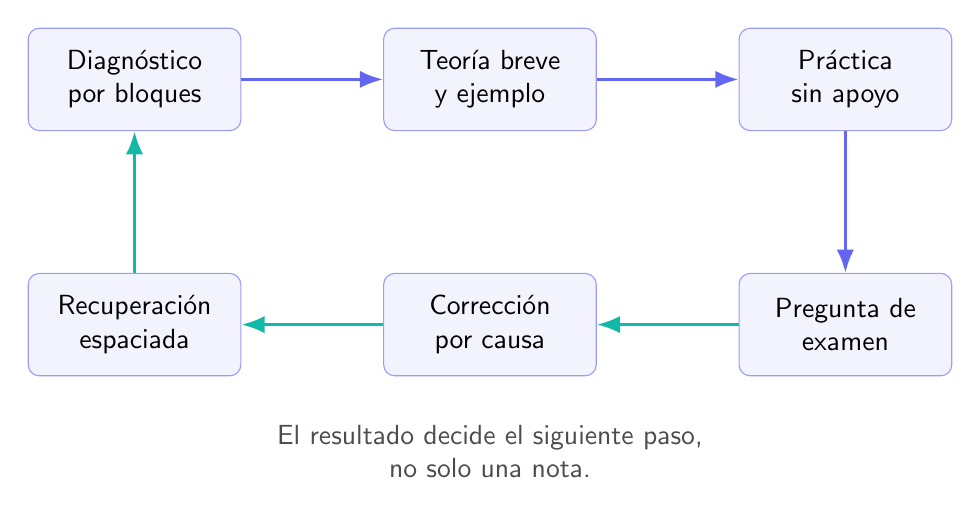
\begin{tikzpicture}[font=\sffamily,>=Latex,node distance=18mm]
  \tikzset{stage/.style={rounded corners=4pt,draw=nebula!65,fill=nebula!8,minimum width=27mm,minimum height=13mm,align=center}}
  \node[stage] (d) {Diagn\'ostico\\por bloques};
  \node[stage,right=of d] (t) {Teor\'ia breve\\y ejemplo};
  \node[stage,right=of t] (p) {Pr\'actica\\sin apoyo};
  \node[stage,below=of p] (e) {Pregunta de\\examen};
  \node[stage,left=of e] (c) {Correcci\'on\\por causa};
  \node[stage,left=of c] (r) {Recuperaci\'on\\espaciada};
  \draw[->,very thick,nebula] (d)--(t);
  \draw[->,very thick,nebula] (t)--(p);
  \draw[->,very thick,nebula] (p)--(e);
  \draw[->,very thick,spark] (e)--(c);
  \draw[->,very thick,spark] (c)--(r);
  \draw[->,very thick,spark] (r)--(d);
  \node[below=5mm of c,align=center,text=black!70] {El resultado decide el siguiente paso,\\no solo una nota.};
\end{tikzpicture}
\end{document}
